\documentclass[]{article}
\usepackage{fontspec}
%\setmainfont{Arial}[ItalicFont={Arial Italic}]
%\setmainfont{Gill Sans MT}[ItalicFont={Gill Sans MT Italic}]
\usepackage[utf8]{inputenc}
\usepackage[margin=1.5cm, bindingoffset=1cm]{geometry}
\linespread{1.5}
\usepackage{float}
\usepackage{csquotes}
\usepackage{subfig}
\usepackage{graphicx}
\usepackage{wrapfig}
\usepackage{xcolor}
\usepackage{indentfirst}
\setlength{\parindent}{0cm}
\usepackage[italian]{babel}
\usepackage{amsmath,amssymb}
\usepackage{hyperref}
\usepackage{amsmath}
\usepackage{enumerate}
\usepackage{enumitem}
\setlist[enumerate]{align=left}
% Imposto colore hyperlinks
\hypersetup{
    colorlinks=true,
    linkcolor=blue,
    urlcolor=blue,
    }
\usepackage{color}
\usepackage{listings}
\usepackage{wrapfig}
\usepackage{url}

\lstset{showstringspaces=false}

\title{CCFDetector}
\author{Marco Santoriello}
\date{Gennaio 2024}

\begin{document}
\begin{titlepage}
    \begin{center}
        \LARGE{\uppercase{Università degli Studi di Salerno}}\\
        \vspace{5mm}
        %Dipartimento
    	\uppercase{\normalsize Dipartimento di Informatica}\\
    \end{center}
    \begin{figure}[H]
        \centering
        
\includegraphics[width=0.35\textwidth]{img/logo_unisa.png}
    \end{figure}

    \begin{center}
        %Corso di Laurea
    	\normalsize{ Corso di Laurea in informatica }\\
    	\vspace{15mm}
    	%Titolo
        {\LARGE{\bf CCFDetector: Using ML against Credit Card Frauds }}\\
        {\large{ Progetto realizzato per l'esame di Fondamenti di Intelligenza Artificiale}}\\
    	\vspace{10mm}
    \end{center}
    \begin{minipage}[t]{0.4\textwidth}\raggedright
        %Candidato
    	{\large{Scritto da: \\ \bf Marco Santoriello\\ Mat. 0512114100}}
    \end{minipage}

    \vspace{90mm}
    %Anno Accademico
    \centering{\large \uppercase{ Anno Accademico 2023/2024 }}

\end{titlepage}

\setcounter{tocdepth}{3} %IMPOSTO LIVELLO PROFONDITA' INDICE

\tableofcontents
\newpage


\section{Introduzione}
    Negli ultimi anni, sempre più piede hanno preso i pagamenti elettronici, al punto che, anche in Italia, per legge, ogni commerciante deve essere munito di un dispositivo che permetta al cliente di pagare utilizzando la propria carta di credito, rischiando, in caso di mancato adempimento a questa legge, ingenti sanzioni pecuniarie.\\
    Come è facile immaginare, questo cambiamento nel modo in cui il denaro viene messo in circolazione ha interessato notevolmente criminali e truffatori (i cosiddetti \textit{scammers}), i quali hanno trovato non pochi modi di impossessarsi illecitamente, in maniera fisica o meno, delle carte di credito altrui.
    Basti pensare che negli Stati Uniti, secondo la \textit{Federal Trade Commission}, la tipologia di furti di identità più diffusi è proprio correlata alle frodi relative alle carte di credito.\\
    Queste frodi possono avvenire in svariati modi: si parte dal furto vero e proprio della carta di credito, fino ad arrivare, tramite diversi metodi, all'appropriazione dei soli dati della carta che abilitano al pagamento, passando per la clonazione delle carte e per l'utilizzo di dispositivi \textit{contactless} in posti affollati in prossimità dei portafogli delle ignare vittime.\\
    Questo progetto nasce con lo scopo di addestrare un modello di Machine Learning che permetta una facile ed affidabile individuazione delle transazioni fraudolente, con lo scopo di bloccarle tempestivamente per evitare sottrazioni di denaro alle vittime.

    \subsection{Specifica PEAS}
        La specifica PEAS (Performance, Environment, Actuators, Sensors) è un sistema che permette di descrivere l'ambiente operativo di un agente intelligente. L'obiettivo principale del progetto è quello di massimizzare la capacità dell'agente di rilevare transazioni fraudolente. L'ambiente in cui l'agente dovrà operare è di seguito descritto:
        \begin{itemize}
            \item Performance:
            \item Environment:
            \item Actuators:
            \item Sensors:
        \end{itemize}

    \subsection{Caratteristiche dell'ambiente}
        % TO-DO

    \subsection{Analisi del Problema}
        %TO-DO

\section{Data Understanding}
    \subsection{Data Collection}
        Definito il Problem Statement, passo all'individuazione del dataset adatto per l'addestramento e la validazione del modello.\\
        Trattandosi di dati particolarmente sensibili, il numero di dataset presenti online non è molto alto. Il primo \href{https://www.kaggle.com/datasets/mlg-ulb/creditcardfraud}{dataset} ritenuto particolarmente interessante per gli scopi di questo progetto, risultava avere quasi tutte le features criptate (per ovvi motivi di privacy) e delle quali non veniva fornita alcuna spiegazione, trattandosi di transazioni reali, rivelandosi non ottimale in termini di explainability.
        La scelta è poi ricaduta su un \href{https://www.kaggle.com/datasets/ealtman2019/credit-card-transactions/data}{dataset} contenente dati simulati, rilasciato da IBM.

    \subsection{Data Description}
        Il dataset in questione comprende dati, ottenuti attraverso un processo di simulazione che non è stato reso noto, di oltre 24 milioni di transazioni, di cui 30.000 fraudolente (cioè lo 0.1\%). Essendo dati simulati, ci si aspetta siano fedeli rappresentazioni delle transazioni reali e delle loro caratteristiche.\\
        Le features di questo dataset comprendono tutti i dettagli relativi a un pagamento elettronico (ID utente, ID carta, data, ora, modalità di pagamento, ecc.) e tutti i dettagli del venditore (i cui nomi sono stati codificati). La variabile target è rappresentata dalla colonna \textit{Is Fraud?}.\\
        Per ragioni legate alla capacità dell'hardware, decido di caricare soltanto 300.000 righe del dataset, verificando subito la presenza di transazioni fraudolente tra quelle importate.
        Procedo, a questo punto, con la documentazione dei dati.\\
        Il dataset contiene 15 colonne che riporto di seguito, associando ad ognuna una breve descrizione di essa:
        \begin{enumerate}[label=\roman*.]
            \item \textbf{User}: Id dell'utente che ha effettuato la transazione (Dtype: int64)
            \item \textbf{Card}: Id della carata che ha effettuato la transazione (Dtype: int64)
            \item \textbf{Year}: Anno in cui è avvenuta la transazione (Dtype: int64)
            \item \textbf{Month}: Mese in cui è avvenuta la transazione (Dtype: int64)
            \item \textbf{Day}: Giorno in cui è avvenuta la transazione (Dtype: int64)
            \item \textbf{Time}: Istante in cui è avvenuta la transazione (Dtype: object)
            \item \textbf{Amount}: Ammontare (in dollari) della transazione (Dtype: object)
            \item \textbf{Use Chip}: Modalità di pagamento (Dtype: object)
            \item \textbf{Merchant Name}: Nome del venditore presso cui si ha acquistato (Dtype: int64)
            \item \textbf{Merchant City}: Città del venditore presso cui si ha acquistato (Dtype: object)
            \item \textbf{Merchant State}: Stato del venditore presso cui si ha acquistato (Dtype: object)
            \item \textbf{Zip}: Zip code del venditore presso cui si ha acquistato (Dtype: float64)
            \item \textbf{MCC}: Merchant Category Code (Dtype: int64)
            \item \textbf{Errors?}: Se è avvenuto un errore, ne descrive la tipologia (Dtype: object)
            \item \textbf{Is Fraud?}: Transazione fraudolenta oppure lecita (Dtype: object)
        \end{enumerate}
        Per quanto riguarda le modalita' di pagamento, rappresentate nella colonna \textit{Use Chip}, osservo che sono di tre tipi:
        \begin{itemize}
            \item [-] \textit{Chip Transaction}: pagamento effettuato inserendo la carta, dotata di chip, nel lettore del terminale POS. Il chip, affinché la transazione possa essere autorizzata, richiede l'inserimento di un codice PIN.
            \item [-] \textit{Swipe Transaction}: pagamento effettuato utilizzando la striscia magnetica della carta. Tale tipologia di pagamento non prevede l'inserimento del PIN (perlomeno se il pagamento è al di sotto di una determinata soglia) per autorizzare la transazione.
            \item [-] \textit{Online Transaction}: pagamento online, effettuato inserendo i dati della carta manualmente, all'interno di un form. Anche in questo caso, a seconda dell'importo della transazione, potrebbe essere richiesta una misura di sicurezza aggiuntiva, oppure no.
        \end{itemize}
        Per poter continuare ad esplorare i dati, devo effettuare delle operazioni di conversione e splitting, anticipando, così, la fase di \textbf{data cleaning}.
        Innanzitutto, la feture \textit{Amount}, contenente l'importo di ogni transazione in dollari, non risulta essere in formato numerico, per cui vado a convertirne tutti i suoi valori in float, non prima di aver rimosso il simbolo della valuta che precede le cifre.\\
        Gestisco, poi, la caratteristica \textit{Time} che provvedo a dividere nelle caratteristiche \textit{Hour} e \textit{Minute}, rimuovendola, infine, dal dataset.
        Vado ora ad analizzare la distribuzione delle varie features, per cercare di capire meglio eventuali patterns legati con le frodi.\\
        In particolare, dal seguente grafico, osservo che la maggior parte degli importi che caratterizzano le transazioni fraudolente sono relativamente bassi, compresi, infatti nell'intervallo che va da 0 a 250 USD.
        \begin{figure}[H]
            \centering
            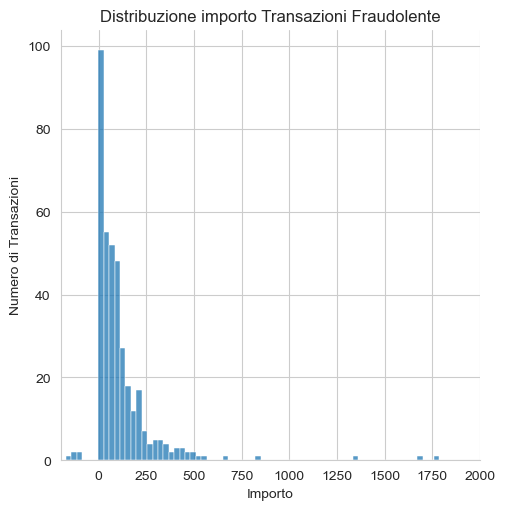
\includegraphics[width=.4\textwidth]{img/DistribuzioneImporto.png}
            \caption[short]{Distrubuzione degli importi relativi alle transazioni fraudolente}
        \end{figure}
        Inoltre, il metodo di pagamento maggiormente interessato da questo fenomeno, risulta essere il pagamento online. Invece, come mi aspettavo dalla precedente analisi fatta sui metodi di pagamento, quello tramite chip risulta essere il meno interessato, rivelandosi, dunque, il metodo piu' sicuro.
        \begin{figure}[H]
            \centering
            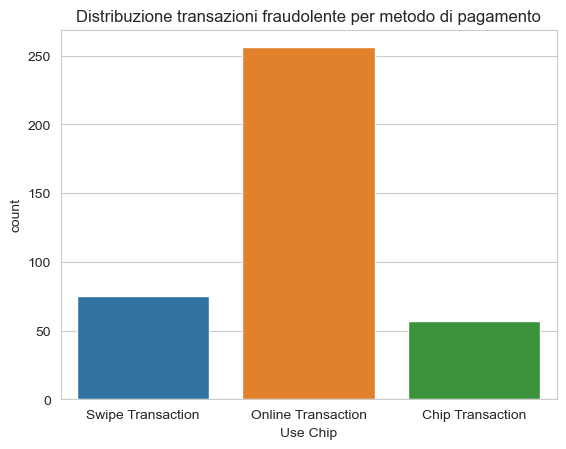
\includegraphics[width=.4\textwidth]{img/DistribuzioneMetodoPagamento.png}
            \caption[short]{Distribuzione dei metodi di pagamento}
        \end{figure}

    \subsection{Data Quality}
        Relativamente alla qualità dei dati, la prima cosa che noto è che le colonne \textit{Merchant State}, \textit{Zip}, ed, in particolare \textit{Errors}, contengono dei valori nulli.
        \begin{figure}[H]
            \centering
            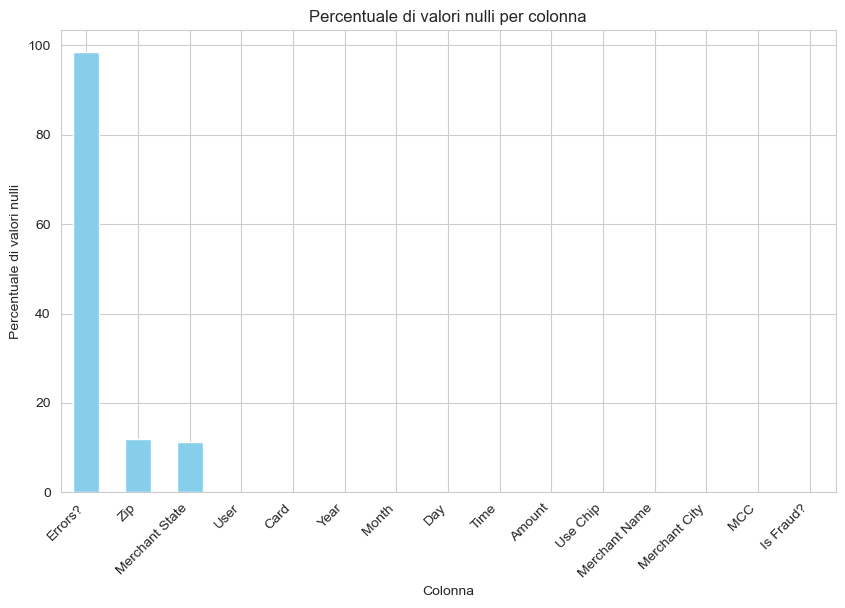
\includegraphics[width=.6\textwidth]{img/NullValuesPercentage.png}
            \caption[short]{Percentuale valori nulli per colonna}
        \end{figure}
        Inoltre, le caratteristiche \textit{Merchant State} e \textit{Zip} possono essere ricavate da \textit{Merchant City}, dunque potrebbe essere conveniente, contenendo valori nulli, rimuoverle.
        Procedo, dunque, a verificare è se il dataset è bilanciato o meno. Il numero di transazioni fraudolente è pari a 388, cioe' lo 0.129\% del totale delle transazioni. Il dataset risulta essere altamente sbilanciato, come mostrato dal seguente grafico:
        \begin{figure}[H]
            \centering
            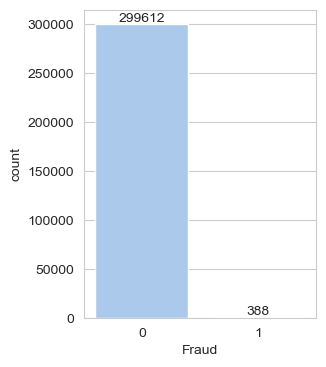
\includegraphics[width=.4\textwidth]{img/DistribuzioneFraudVsGen2.png}
            \caption[short]{Distrubuzione delle transazioni fraudolente e lecite}
        \end{figure}
        L’utilizzo di un dataset così sbilanciato, porterebbe alla costruzione di un modello altamente impreciso e che, probabilmente, si \textit{adatterà troppo} (\textit{overfitting}) al problema, in quanto andrebbe ad assumere la maggior parte delle transazioni come non fraudolente, siccome queste costituiscono la stragrande maggioranza dei dati.

\section{Data Preparation}
    In questa fase, vado ad effettuare le operazioni necessare per la pulizia dei dati, in modo che possano essere pronti per essere dati in input al modello.
    \subsection{Data Cleaning}
        Innanzitutto vado a gestire i valori nulli. Parto dalla caratteristica \textit{Errors?}. Come analizzato in fase di Data Understanding, questa colonna contiene le varie tipologie di errore a cui una transazione puo' andare incontro.
        \begin{center}
            \begin{tabular}{|c|}
                \hline
                \textbf{Errors?}\\
                \hline
                NaN\\
                \hline
                Bad Pin\\
                \hline
                Insufficient Balance\\
                \hline
                Technical Glitch\\
                \hline
                Bad Card Number\\
                \hline
                Bad CVV\\
                \hline
                Bad Expiration\\
                \hline
                Bad Zipcode\\
                \hline
                Insufficient Balance,Technical Glitch\\
                \hline
                Bad Card Number,Bad CVV\\
                \hline
            \end{tabular}
        \end{center}
        Come risulta dall'osservazione dei valori di questa feature, i valori nulli sembrano corrispondere al caso in cui non si verifica alcun errore. Per tale ragione, decido di rimpiazzare tutti i valori nulli con il valore \textit{No error}. Tale modo di gestire i valori nulli si definisce \textbf{imputazione deduttiva}.\\
        Come secondo step, vado a rimuovere le colonne \textit{Merchant State} e \textit{Zip}. Esse, infatti, posso essere ricavate dalla feature \textit{Merchant City}, per cui, contenendo specialmente dei valori nulli, risulta conveniente la loro rimozione dal dataset.\\
        Necessitando per il futuro addestramento del modello di dati numerici, vado a convertire le variabili categoriche \textit{Use Chip}, \textit{Merchant City} ed \textit{Errors} in variabili numeriche, utilizzando il metodo \textbf{LabelEncoder()}, della libreria \textit{scikit-learn}. Tale metodo assegna un intero univoco ad ogni categoria, in ordine di scoperta.
    \subsection{Feature Scaling}
        Nella fase di Feature Scaling, proseguo con l'osservazione delle distribuzioni dei valori delle varie caratteristiche, poiché addestrare un modello su un dataset che contiene colonne con insiemi di valori molto diversi tra loro, potrebbe portare tale modello a confondersi, sovrastimando o sottostimando l'importanza delle varie caratteristiche.\\
        Le varie features, tra loro, assumono valori compresi in diversi ranges, per tale ragione, decido di effettuare la normalizzazione su tutte, tranne che sulla variabile dipendente.\\
        Per lo scopo, utilizzo la tecnica di \textbf{Normalizzazione min-max}, che è una delle più comuni e diffuse tecniche di normalizzazione.
        Di seguito riportata la formula della Normalizzazione min-max:
        \begin{center}
            \[
                x_{\text{norm}} = a + \frac{{x - \min(X)}}{{\max(X) - \min(X)}} \cdot (b - a)
            \]
        \end{center}
        Normalizzati i valori, passo alla fase di Feature Selection.
    \subsection{Feature Selection}


\end{document}